\begin{frame}[t]
\frametitle{Semidiscrete problem}
\begin{block}{FEM equations}
\begin{overlayarea}{\textwidth}{2.0cm}
\vspace{-0.8cm}
\begin{align*}
% FEM EQUATIONS
\left( \mathbf{v}_{h},\partial _{t}\mathbf{u}_{h}\right) _{\Omega }
+ b\left(\mathbf{a},\mathbf{u}_h, \mathbf{v}_h\right)
+\left( \mathbf{\nabla v}_{h},\nu \mathbf{\nabla u}_{h}\right) _{\Omega} &
-\left( \mathbf{\nabla }\cdot \mathbf{v}_{h},p_{h}\right) _{\Omega }
\\[0.05in]
\onslide<1>{+\left( \mathbf{v}_{h},\partial _{t}\widetilde{\mathbf{u}}\right) _{\Omega}}
\alert<2->{+\left( \mathcal{L}^{\ast }\mathbf{v}_{h},\widetilde{\mathbf{u}}\right)_{\Omega^h}
-\left( \mathbf{\nabla }\cdot \mathbf{v}_{h},\widetilde{p}\right) _{\Omega^h}} &
=\left\langle \mathbf{v}_{h},\mathbf{f}\right\rangle_{\Omega }
\\[0.1in]
\left( q_{h},\mathbf{\nabla }\cdot \mathbf{u}_{h}\right) _{\Omega }
\alert<2->{-\left( \mathbf{\nabla }q_{h},\widetilde{\mathbf{u}}\right) _{\Omega^h}} & =0
\end{align*}
\end{overlayarea}
\end{block}
\begin{block}{SGS equations}
\vspace{-0.4cm}
\begin{align*}
% SGS EQUATIONS
\onslide<1>{\partial_{t}\widetilde{\mathbf{u}} +} \alert<2->{\tau_{m}^{-1} \widetilde{\mathbf{u}}}
&= \alert<2->{\mathcal{P} \mathbf{R}_{m}}
\\[0.05in]
%\\[0.1in]
\tau _{c}^{-1} \widetilde{p} & = \mathcal{P} R_{c}
\end{align*}
\end{block}
%\end{overlayarea}
\vspace{-0.2cm}
\begin{overlayarea}{\textwidth}{3.0cm}
\begin{equation*}
\onslide<1>{\mathcal{P} = I \quad \rm{(ASGS)},} \quad \quad \alert<2->{\mathcal{P} = P_h^{\perp}=I-P_h \quad \rm{(OSS)}}
\end{equation*}
\vspace{-0.2cm}
\begin{equation*}
\alert<2->{\mathbf{a=u}_{h}}\onslide<1>{+\widetilde{\mathbf{u}}}
\end{equation*}
\end{overlayarea}
\end{frame}
%----------------------------------------------------------------------------------------
\begin{frame}[t]
\frametitle{Term-by-term OSS}
\only<1>{
\begin{block}{FEM equations}
\begin{overlayarea}{\textwidth}{6.0cm}
\vspace{-0.8cm}
\begin{align*}
% FEM EQUATIONS
\left( \mathbf{v}_{h},\partial _{t}\mathbf{u}_{h}\right) _{\Omega }
+ b\left(\mathbf{a},\mathbf{u}_h, \mathbf{v}_h\right)
+\left( \mathbf{\nabla v}_{h},\nu \mathbf{\nabla u}_{h}\right) _{\Omega} &
-\left( \mathbf{\nabla }\cdot \mathbf{v}_{h},p_{h}\right) _{\Omega }
\\[0.05in]
\onslide<0>{+\left( \mathbf{v}_{h},\partial _{t}\widetilde{\mathbf{u}}\right) _{\Omega}}
\alert<1->{+\left( \mathcal{L}^{\ast }\mathbf{v}_{h},\widetilde{\mathbf{u}}\right)_{\Omega^h}
-\left( \mathbf{\nabla }\cdot \mathbf{v}_{h},\widetilde{p}\right) _{\Omega^h}} &
=\left\langle \mathbf{v}_{h},\mathbf{f}\right\rangle_{\Omega }
\\[0.1in]
\left( q_{h},\mathbf{\nabla }\cdot \mathbf{u}_{h}\right) _{\Omega }
\alert<1->{-\left( \mathbf{\nabla }q_{h},\widetilde{\mathbf{u}}\right) _{\Omega^h}} & =0
\end{align*}
\end{overlayarea}
\end{block}}
\only<2->{
\begin{block}{Term-by-term OSS (Codina 2008)}
\begin{overlayarea}{\textwidth}{6.0cm}
\vspace{-0.8cm}
\begin{align*}
&\left( \mathbf{v}_{h},\partial _{t}\mathbf{u}_{h}\right) _{\Omega }
+ b\left(\mathbf{a},\mathbf{u}_h, \mathbf{v}_h\right)
+\left( \mathbf{\nabla v}_{h},\nu \mathbf{\nabla u}_{h}\right) _{\Omega} 
-\left( \mathbf{\nabla }\cdot \mathbf{v}_{h},p_{h}\right) _{\Omega }
\\[0.05in]
&+\only<2>{\alert<2>{\left(\tau_m \mathbf{a}\cdot\nabla\mathbf{v}_{h},\mathcal{P}_h^\perp(\mathbf{a}\cdot\nabla\mathbf{u}_{h})\right)_{\Omega^h}}}
\only<3>{\alert<3>{\left(\tau_m \mathbf{a}\cdot\nabla\mathbf{v}_{h},\mathbf{a}\cdot\nabla\mathbf{u}_{h}\right)_{\Omega^h}-\left(\tau_m \mathbf{a}\cdot\nabla\mathbf{v}_{h},\boldsymbol{\eta}_{h}\right)_{\Omega^h}}}\\
&+\alert<2-3>{\left(\tau_c \nabla\cdot\mathbf{v}_{h},\nabla\cdot\mathbf{u}_{h}\right) _{\Omega^h}} 
=\left\langle \mathbf{v}_{h},\mathbf{f}\right\rangle_{\Omega }
\\[0.1in]
%
&\left( q_{h},\mathbf{\nabla }\cdot \mathbf{u}_{h}\right) _{\Omega }
+\only<2>{\alert<2>{\left(\tau_m \nabla q_{h},\mathcal{P}_h^\perp(\nabla p_{h})\right) _{\Omega^h}} }
\only<3>{\alert<3>{\left(\tau_m \nabla q_{h},\nabla p_{h}\right) _{\Omega^h}-\left(\tau_m \nabla q_{h},\boldsymbol{\xi}_{h}\right) _{\Omega^h}}}
 =0
\end{align*}
\only<3->{
\begin{align*}
&\boldsymbol{\eta}_{h}:=\mathcal{P}_h(\mathbf{a}\cdot\nabla\mathbf{u}_{h})\\
&\boldsymbol{\xi}_{h}:=\mathcal{P}_h(\nabla p_{h})
\end{align*}}
\end{overlayarea}
\end{block}}
\end{frame}
%----------------------------------------------------------------------------------------
\begin{frame}
\frametitle{Matrix form}
%\begin{overlayarea}{\textwidth}{6.0cm}
\begin{itemize}
\item<1-> ASGS:
\begin{equation*}
\left[\begin{array}{c}
M\dot{\U}\\
\mathbf{0}
\end{array}\right]+\left[\begin{array}{cc}
K+C+A_\tau&G+G_\tau\\
D+D_\tau&L_\tau
\end{array}\right]\left[\begin{array}{c}
\U\\
\P
\end{array}\right]=\left[\begin{array}{c}
\F_u\\
\mathbf{G}
\end{array}\right],
\end{equation*}
\item<2-> Term-by-term OSS:
\begin{equation*}
\left[\begin{array}{c}
M\dot{\U}\\
\mathbf{0}\\
\mathbf{0}\\
\mathbf{0}
\end{array}\right]+\left[\begin{array}{cccc}
K+C+A_\tau&G&B_{\eta,\tau}&0\\
D&L_\tau&0&B_{\xi,\tau}\\
-B_{\eta,\tau}^T&0&M_{\eta,\tau}&0\\
0&-B_{\xi,\tau}^T&0&M_{\xi,\tau}
\end{array}\right]\left[\begin{array}{c}
\U\\
\P\\
\ETA\\
\XI
\end{array}\right]=\left[\begin{array}{c}
\F_u\\
\mathbf{G}\\
\mathbf{0}\\
\mathbf{0}
\end{array}\right],
\end{equation*}
\item<3-> Term-by-term OSS with Inf-sup stable elements (mixed FE):
\begin{equation*}
\left[\begin{array}{c}
M\dot{\U}\\
\mathbf{0}\\
\mathbf{0}
\end{array}\right]+\left[\begin{array}{ccc}
K+C+A_\tau&G&B_\tau\\
D&\alert<4>{0}&0\\
-B_\tau^T&0&M_\tau
\end{array}\right]\left[\begin{array}{c}
\U\\
\P\\
\ETA
\end{array}\right]=\left[\begin{array}{c}
\F_u\\
\mathbf{G}\\
\mathbf{0}
\end{array}\right],
\end{equation*}
\end{itemize}
\vspace{-0.2cm}
\onslide<4>{\begin{center}
\alert<4>{Index-2 DAE!!!}
\end{center} }
%\end{overlayarea}
\end{frame}
%%----------------------------------------------------------------------------------------
%\begin{frame}
% \frametitle{TGV {\small Taylor-Green Vortex flow}}
% \textbf{Energy dissipation rate (different methods):}
% \begin{itemize}
% 	\itemsep-0.1cm
%  	\item Different mesh discretizations for ASGS and OSS ($ Q_1/Q_1 $,$ Q_2/Q_2 $)
%  	\item $ Q_2/Q_1 $ discretization for mixed FE OSS.
% \end{itemize}
% \vspace*{-0.5cm}
% \begin{figure}
%     \centering	
%     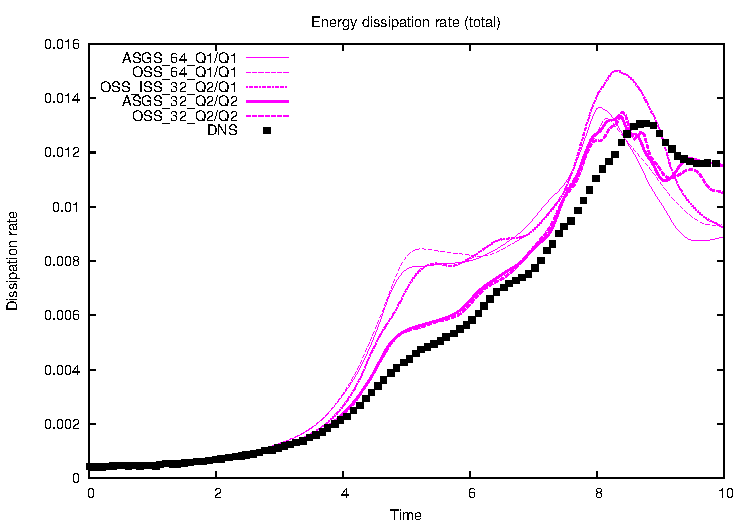
\includegraphics[width=0.6\textwidth]{Figures/oss_64_tot.pdf}
%     \vspace*{-0.2cm}
% \end{figure}
% \begin{overlayarea}{\textwidth}{1.5cm}
% \only<2->{
% \vspace*{-0.5cm}
% \begin{itemize}
% 	\itemsep-0.1cm
%  	\item \alert<2>{Good agreement with the DNS} (coarse mesh).
%  	\only<3->{\item \alert<3>{More accurate results with equal-order elements}.}
%  \end{itemize}}
%  \end{overlayarea}
%\end{frame}
%%----------------------------------------------------------------------------------------
%\begin{frame}
% \frametitle{TGV {\small Taylor-Green Vortex flow}}
% \textbf{Computational cost (different methods):}
% \begin{itemize}
% 	\itemsep-0.1cm
%  	\item Acumulated solver iterations.
% \end{itemize}
% \vspace*{-0.5cm}
% \begin{figure}
%     \centering	
%     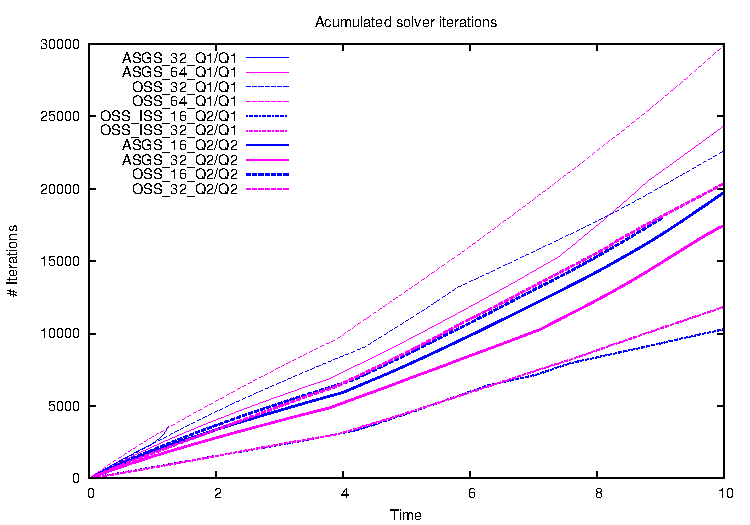
\includegraphics[width=0.7\textwidth]{Figures/oss_all_acu.pdf}
%     \vspace*{-0.2cm}
% \end{figure}
% \begin{overlayarea}{\textwidth}{1.5cm}
% \only<2->{
% \vspace*{-0.5cm}
% \begin{itemize}
% 	\itemsep-0.1cm
%  	\item \alert<2>{Mixed FE OSS cheapest}.
%  \end{itemize}}
%  \end{overlayarea}
%\end{frame}
%%----------------------------------------------------------------------------------------
%\begin{frame}
%\frametitle{Mixed FE OSS Conclusions}
%\begin{itemize}
%\item<1-> Better results for equal-order interpolations.
%\item<2-> Mixed FE OSS the cheapest method.
%\item<3-> Mixed FE OSS $ Q_2/Q_1 $ better and cheaper than other methods with $ Q_1/Q_1 $. 
%\end{itemize}
%\end{frame}